\documentclass[laboratorio]{guia}

\def \practnum {8}
\def \practica {Interferencia: Biprisma de Fresnel}

\def \materia {Laboratorio de F\'\i sica II para Qu\'\i micos}
\def \periodo {2\sptext{o} cuatrimestre de 2016}
\def \profesor {Diana Skigin}
\def \website {http://materias.df.uba.ar/f2qa2016c2}

\usepackage{graphics}
\usepackage{amsmath}
\usepackage{amsfonts}
\usepackage{graphicx}
\usepackage{float}
\usepackage{wrapfig}
\usepackage{subfigure}
\usepackage{bm}
\usepackage{grffile}
\usepackage{color}
\usepackage{framed}
\usepackage[utf8]{inputenc}
\usepackage[T1]{fontenc}
\usepackage{lmodern}
% definicion del entorno 'sabermas'
\makeatletter
\definecolor{shadecolor}{rgb}{0.89,0.91,0.94}
\newenvironment{sabermas}[1]{%
\vfill
\begin{shaded}
  \begin{center}
  {\textsection{Para saber m\'as}}
  \end{center}
  #1
\sf } 
{%
\end{shaded}%
}
\makeatother

\renewcommand{\vec}[1]{\ensuremath{\mathbf{#1}}}



\hyphenation{ coe-fi-cien-tes coe-fi-cien-te au-to-va-lor
              au-to-va-lo-res co-rres-pon-der pro-ble-ma 
              cual-quie-ra po-la-ri-za-cio-nes }

\graphicspath{{./Guia_09_Interferencia/}}

\begin{document}
\objetivo{%
    La presente gu\'\i a tiene como objetivo determinar la longitud de onda de
    mayor intensidad emitida por una l\'ampara de Sodio, empleando para ello un
    m\'etodo interferom\'etrico.
    \tematicas{interferencia, dos rendijas, biprisma de Fresnel, espectro de
        emisi\'on del Sodio, doblete del Sodio. }}
\maketitle

\section{Introducci\'on}

El biprisma de Fresnel es un interfer\'ometro por divisi\'on de frente de onda
similar al experimento de la doble rendija de Young. El mismo consta de dos
prismas delgados que sirven para generar dos im\'agenes coherentes de una
\'unica fuente (una rendija iluminada) de modo tal que la luz proveniente de
ambas da lugar a interferencia en la zona situada a continuaci\'on del
biprisma. Estas franjas son franjas reales {\it no localizadas}, es decir que
pueden verse sobre una pantalla en toda una regi\'on que se extiende m\'as
all\'a de la posici\'on del biprisma. Se puede demostrar que el plano donde se
encuentran ubicadas las fuentes virtuales generadas por el biprisma es el mismo
plano en el cual se encuentra dispuesta la rendija. 

En cada punto del espacio donde la diferencia de camino \'optico entre las
ondas provenientes de cada fuente resulte igual a un n\'umero entero de
longitudes de onda habr\'a entonces interferencia constructiva y se ver\'a una
franja brillante. 

M\'as a\'un, es posible mostrar que la separaci\'on entre franjas de interferencia
viene dada por
\begin{equation}
    \delta y = s \frac{\lambda}{a},
    \label{eq:1}
\end{equation}
donde $\delta y$ representa la distancia entre dos m\'aximos brillantes
consecutivos (interfranja), $s$ corresponde a la distancia entre el plano de
las fuentes virtuales y el plano donde se observa el patr\'on de interferencia,
y $a$ denota la distancia entre las dos fuentes virtuales responsables por la
interferencia.

El prop\'osito de la presente experiencia es el de determinar
experimentalmente, a partir de la ecuaci\'on \eqref{eq:1}, la longitud de onda
de mayor intensidad emitida por una l\'ampara de Sodio, que a los efectos
pr\'acticos de esta gu\'\i a se considerar\'a monocrom\'atica.

\section{Desarrollo de la experiencia}

\subsection{Calibraci\'on del microscopio y medici\'on de la distancia de
enfoque}

Dado que la figura de interferencia es muy peque\~na, la misma no puede
observarse a simple vista, por lo que se requiere del uso de un microscopio de
banco. Este elemento \'optico cuenta con un ret\'\i culo que puede desplazarse
empleando una rueda graduada (micr\'ometro), a fin de poder medir los objetos
que yacen dentro de su campo visual.

Antes de poder realizar dichas mediciones es necesario determinar la escala en
la que est\'a graduado el micr\'ometro. Para ello, enfoque con el microscopio
un papel milimetrado y determine experimentalmente a qu\'e distancia equivale
una unidad sobre la escala del micr\'ometro.

Preste particular atenci\'on al hecho de que el micr\'ometro del microscopio
{\bf solo debe rotarse en el mismo sentido}, (sea cual fuere \'este), dado que
el mismo no vuelve sobre sus mismos pasos. 

\begin{figure}[t!]
    \centering
    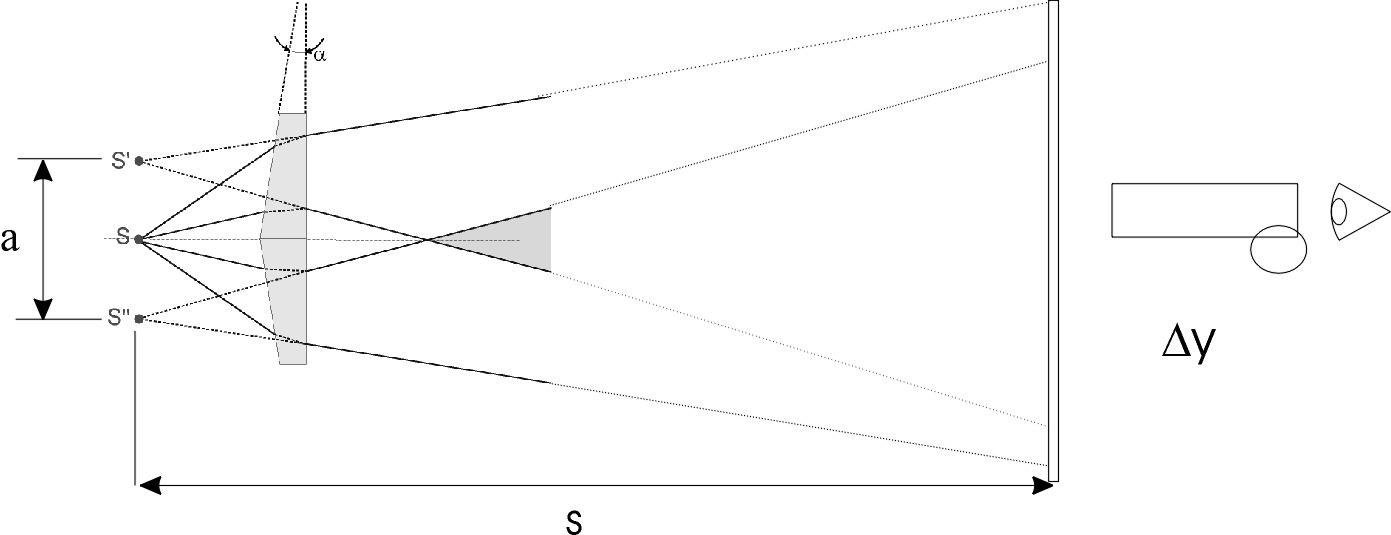
\includegraphics[width=8.5cm]{LG09--000.png}
    \caption{Esquema del montaje sugerido para observar el fen\'omeno de
    interferencia entre dos fuentes puntuales (virtuales).}
    \label{fig:1}
\end{figure}



\subsection{Medici\'on de la longitud de onda de la l\'ampara de Sodio}

Sobre un banco \'optico, coloque el microscopio, el biprisma y la rendija. Note
que puede resultarle conveniente 
ubicar el biprisma en un brazo con desplazamiento lateral
(perpendicular al eje del banco), dado que esta pr\'actica presenta -como
requisito fundamental- disponer de los elementos \'opticos correctamente
alineados. 

Por otro lado, la l\'ampara de Sodio requiere de un tiempo para entrar en
r\'egimen, por lo que conviene prenderla varios minutos antes de comenzar; ya
que de otro modo se estar\'\i an viendo longitudes de onda que no son las que
se busca determinar.

Teniendo en cuenta estas precauciones, comience la experiencia. Para ello,
acerque el microscopio al biprisma y desplace \'este lateralmente hasta ver
ambas fuentes virtuales, las cuales deben aparecer de igual intensidad, ancho
y altura. Desenfoque entonces ligeramente el microscopio y aseg\'urese de que
a\'un en este caso ambas fuentes virtuales contin\'uan presentando las mismas
caracter\'\i sticas. Aleje el microscopio a una distancia donde pueda observar ahora las franjas de
interferencia.

\nocite{Alonso1998,Jenkins2001,Hecht1986}
\bibliographystyle{unsrt} 
\bibliography{Bibliografia}
        

\end{document}
